\documentclass[floatsintext,doc]{apa6}

\usepackage{amssymb,amsmath}
\usepackage{ifxetex,ifluatex}
\usepackage{fixltx2e} % provides \textsubscript
\ifnum 0\ifxetex 1\fi\ifluatex 1\fi=0 % if pdftex
  \usepackage[T1]{fontenc}
  \usepackage[utf8]{inputenc}
\else % if luatex or xelatex
  \ifxetex
    \usepackage{mathspec}
    \usepackage{xltxtra,xunicode}
  \else
    \usepackage{fontspec}
  \fi
  \defaultfontfeatures{Mapping=tex-text,Scale=MatchLowercase}
  \newcommand{\euro}{€}
\fi
% use upquote if available, for straight quotes in verbatim environments
\IfFileExists{upquote.sty}{\usepackage{upquote}}{}
% use microtype if available
\IfFileExists{microtype.sty}{\usepackage{microtype}}{}

% Table formatting
\usepackage{longtable, booktabs}
\usepackage{lscape}
% \usepackage[counterclockwise]{rotating}   % Landscape page setup for large tables
\usepackage{multirow}		% Table styling
\usepackage{tabularx}		% Control Column width
\usepackage[flushleft]{threeparttable}	% Allows for three part tables with a specified notes section
\usepackage{threeparttablex}            % Lets threeparttable work with longtable

% Create new environments so endfloat can handle them
% \newenvironment{ltable}
%   {\begin{landscape}\begin{center}\begin{threeparttable}}
%   {\end{threeparttable}\end{center}\end{landscape}}

\newenvironment{lltable}
  {\begin{landscape}\begin{center}\begin{ThreePartTable}}
  {\end{ThreePartTable}\end{center}\end{landscape}}




% The following enables adjusting longtable caption width to table width
% Solution found at http://golatex.de/longtable-mit-caption-so-breit-wie-die-tabelle-t15767.html
\makeatletter
\newcommand\LastLTentrywidth{1em}
\newlength\longtablewidth
\setlength{\longtablewidth}{1in}
\newcommand\getlongtablewidth{%
 \begingroup
  \ifcsname LT@\roman{LT@tables}\endcsname
  \global\longtablewidth=0pt
  \renewcommand\LT@entry[2]{\global\advance\longtablewidth by ##2\relax\gdef\LastLTentrywidth{##2}}%
  \@nameuse{LT@\roman{LT@tables}}%
  \fi
\endgroup}


  \usepackage{graphicx}
  \makeatletter
  \def\maxwidth{\ifdim\Gin@nat@width>\linewidth\linewidth\else\Gin@nat@width\fi}
  \def\maxheight{\ifdim\Gin@nat@height>\textheight\textheight\else\Gin@nat@height\fi}
  \makeatother
  % Scale images if necessary, so that they will not overflow the page
  % margins by default, and it is still possible to overwrite the defaults
  % using explicit options in \includegraphics[width, height, ...]{}
  \setkeys{Gin}{width=\maxwidth,height=\maxheight,keepaspectratio}
\ifxetex
  \usepackage[setpagesize=false, % page size defined by xetex
              unicode=false, % unicode breaks when used with xetex
              xetex]{hyperref}
\else
  \usepackage[unicode=true]{hyperref}
\fi
\hypersetup{breaklinks=true,
            pdfauthor={},
            pdftitle={Quantifying the benefits of using decision models with reaction time and accuracy data},
            colorlinks=true,
            citecolor=blue,
            urlcolor=blue,
            linkcolor=black,
            pdfborder={0 0 0}}
\urlstyle{same}  % don't use monospace font for urls

\setlength{\parindent}{0pt}
%\setlength{\parskip}{0pt plus 0pt minus 0pt}

\setlength{\emergencystretch}{3em}  % prevent overfull lines


% Manuscript styling
\captionsetup{font=singlespacing,justification=justified}
\usepackage{csquotes}
\usepackage{upgreek}



\usepackage{tikz} % Variable definition to generate author note

% fix for \tightlist problem in pandoc 1.14
\providecommand{\tightlist}{%
  \setlength{\itemsep}{0pt}\setlength{\parskip}{0pt}}

% Essential manuscript parts
  \title{Quantifying the benefits of using decision models with reaction time and
accuracy data}

  \shorttitle{Power gains of decision modelling}


  \author{Tom Stafford\textsuperscript{1}, Angelo Pirrone\textsuperscript{2}, Mike Croucher\textsuperscript{3}, \& Anna Krystalli\textsuperscript{4}}

  % \def\affdep{{"", "", "", ""}}%
  % \def\affcity{{"", "", "", ""}}%

  \affiliation{
    \vspace{0.5cm}
          \textsuperscript{1} Department of Psychology, University of Sheffield\\
          \textsuperscript{2} School of Psychological and Cognitive Sciences, Peking University\\
          \textsuperscript{3} Research Computing, University of Leeds\\
          \textsuperscript{4} Research Software Engineering, University of Sheffield  }

  \authornote{
    Address correspondance to
    \href{mailto:t.stafford@sheffield.ac.uk}{\nolinkurl{t.stafford@sheffield.ac.uk}}
    
    Correspondence concerning this article should be addressed to Tom
    Stafford, Department of Psychology, University of Sheffield, 1 Vicar
    Lane, Sheffield, S1 2LT, UK. E-mail:
    \href{mailto:t.stafford@sheffield.ac.uk}{\nolinkurl{t.stafford@sheffield.ac.uk}}
  }


  \abstract{Across diverse subfields experimentalists collect reaction time and
accuracy data. Inter-subject and inter-group speed-accuracy trade-offs
(SATOs) are a well-known possibility which are often inadequately
addressed. Many experiments focus on a single variable
(e.g.~psychophysics paradigms analysing accuracy alone), or involve a
post-hoc analytic correction (e.g.~dividing accuracy by reaction time).
Models of decision making, such as the drift diffusion model (DDM),
provide a principled account of the decision making process, allowing
the recovery of SATO-unconfounded parameters from observed variables.
For plausible parameters of a typical between-groups experiment we
simulate experimental data, for both real and null group differences,
and for both systematic and null SATOs, and fit the DDM. This exercise
allows us to make a number of concrete recommendations for
experimentalists: we show, in terms of reduction of required sample
size, how decision modelling allows more efficient data collection for
set statistical power; we confirm and depict the non-linear
speed-accuracy relation; we show how much more sensitive accuracy is as
a measure than reaction time.}
  \keywords{keywords \\

    \indent Word count: X
  }





\usepackage{amsthm}
\newtheorem{theorem}{Theorem}
\newtheorem{lemma}{Lemma}
\theoremstyle{definition}
\newtheorem{definition}{Definition}
\newtheorem{corollary}{Corollary}
\newtheorem{proposition}{Proposition}
\theoremstyle{definition}
\newtheorem{example}{Example}
\theoremstyle{definition}
\newtheorem{exercise}{Exercise}
\theoremstyle{remark}
\newtheorem*{remark}{Remark}
\newtheorem*{solution}{Solution}
\begin{document}

\maketitle

\setcounter{secnumdepth}{0}



\section{Abbreviations}\label{abbreviations}

DDM - Drift diffusion model SATO - Speed-accuracy trade-off

\section{Background}\label{background}

\subsection{Speed accuracy trade-offs}\label{speed-accuracy-trade-offs}

Use of inefficiency scores is widespread in some domains, e.g.~visual
search. (Bruyer \& Brysbaert, 2011)

\section{Logic of the current
investigations}\label{logic-of-the-current-investigations}

\subsection{Goal}\label{goal}

To draw the graph of power against sample size, for different levels of
true effect size. Power depends on experiment design, as well as sample
size and effect size. Currently I am assuming a two group experimental
design, and the difference between them gauged with a two-sample t-test
(although for drift the HDDM implements a Bayesian test by directly
analysing the posteria distributions of the fits for the two groups).
Alternatives would be use of Bayesian tests throughout, or also testing
different experimental designs (such as a within-participants design). A
within-participants design is less preferred because the issue of
systemmatically different speed-accuracy trade-offs between condtions
seems, \emph{prima facie}, unlikely.

With this analysis done, the outputs are:

\begin{itemize}
\tightlist
\item
  Code for reproducing the analysis
  \url{https://github.com/tomstafford/ddm_sims}
\item
  Interactive data visualisation / explorer
  \url{https://annakrystalli.shinyapps.io/xspl_power_analyser/}
\item
  Academic paper explaining the above (based on this document)
\end{itemize}

\subsection{Parameter regimes}\label{parameter-regimes}

Because we are not generating an analytic solution we cannot claim that
our findings are true for all situations - for all parameterisations of
the DDM. Indeed, analytic solutions have already been proposed, and
demonstrate the \emph{in theory} superiority of using the DDM over
analysing reaction time or accuracy alone (Palmer, Huk, \& Shadlen,
2005; Stone, 2014). Our aim is merely to show that for some reasonable
choices of DDM parameters using decision modelling is a superior
approach to analysing reaction time or accuracy alone or combining them
in any suboptimal way.

To be able to make this claim of relevance of our simulations to typical
psychology experiments we need to be able to justify that our parameter
choice is plausible for a typical psychology experiment. In order to
establish this I have picked parameters which generate reaction times of
the order of 1 second and accuracy of the order 90\%.

\begin{itemize}
\tightlist
\item
  Note, for high accuracy values t-tests may not be appropriate (they
  are strictly not applicable to proportions anyway, but this may become
  a real issue for values very close to 1 or 0).
\end{itemize}

\subsection{Effect sizes}\label{effect-sizes}

One nuance is that, for our simulations, it is possible to declare the
effect size in \emph{drift rate}. To be explicit, this is the
\emph{Cohen's d} effect size, defined as the difference between the
difference in mean drift rate between the two groups divided by the
standard deviation which defines between subject variability in drift
rate within the group. These parameters are declared, and the individual
drift rates in each similated experiment generated from these
parameters.

For the observed variables, reaction time and accuracy, the effect sizes
can only be observed, not declared, since these arise from the
interaction of the DDM parameters and the DDM model which generates
responses.

So the declared effect size in drift rate produces the observed effect
size in reaction time and accuracy (which differ from each other),
depending on both the level of noise in each simulated experiment, and
the experiment design - specifically on the number of trials per
participant.

Experiment designs which have a higher number of trials per participant
effectively sample the true drift rates more accurately, and so have
effect sizes for reaction time and accuracy which are closer to the
\enquote{true}, declared, effect size in drift rate.

This issue sheds light on why decision modelling is more effective than
analysing reaction time or accuracy alone (because it recovers the
generating parameter, drift, which is more sensitive to group
differences), and why there are differences in power between measuring
reaction time and accuracy (because, presumably, something about the
dynamics of the DDM and the parameter regime we test in mean that these
variables have different effective effect sizes). See Figure
\ref{fig:effectsizes}

\begin{figure}
\centering
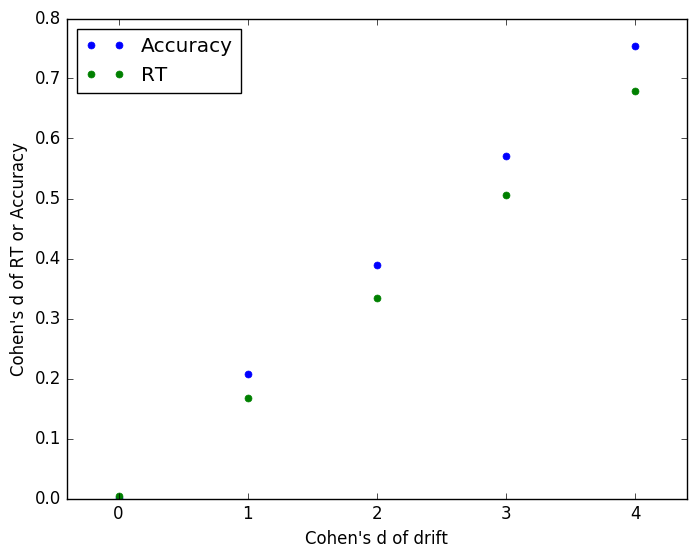
\includegraphics{figs/effectsizetranslation_40trials.png}
\caption{\label{fig:effectsizes}How differences in drift convert to
differences in reaction time and accuracy (10 trials per ppt)}
\end{figure}

\textbf{TODO: Re-run sims with ++ experiments to get RT and Accuracy
effect sizes in the same parameter regime as other sims, for 10, 40, 200
trials.}

\textbf{TODO: explain why, despite observed effect sizes being, for the
most part, comperable, accuracy is more senitive than reaction time}

\subsection{Alpha (false positive
levels)}\label{alpha-false-positive-levels}

Intepreting standard power analysis assumes a standard false positive
(\emph{alpha}) rate of 0.05. It would, for example, be nonsensical to
talk about two tests having an 80\% and 60\% probability, respectively,
of discovering a true effect if we did not know (and hold constant) the
alpha rate (at the limit you can have a power of 100\% if your test
always reports a significant effect - i.e.~an alpha of 1).

For analysing situations where only the drift differs between two groups
this is not a signiicant issue. Our tests have an alpha of 0.05 built in
to them (and, indeed, when the simulations are run the observed false
positive rate does hover around 0.05 as expected).

However, when considering speed-accuracy trade-off changes between
groups (with or without drift rate differences as well) the situation is
different. This means that it is possible to get false positives in
tests of a difference in drifts between groups because of SATOs. Most
obviously, if a SATO means one group prioritises speed over accuracy,
analysis of reaction time alone will mimic an enhanced drift rate, but
analysis of accuracy alone will mimic degraded drift rate. Ideally the
DDM will be immune to distortion of estimate of drift rates, but that is
what we have set out to demonstrate so we should not assume.

The consequence of this is that it makes sense to move from calculating
power for simulated experiments, but to calculate false positive rate as
well - i.e.~to compare the rate of significant differences with and
without true differences in drift. A principled way for combining these
into a single metric is d', which gives an overall sensitivity of the
test, much as we would calculate the sensitivity independent of bias for
an observer in a psychophysics experiment.

\section{Methods}\label{methods}

Ideally we would independently reproduce these results using different
DDM implementations.

For the result reported here I use the HDDM (Wiecki, Sofer, \& Frank,
2013), running under the Anaconda distribution of Python 3. Code is here
\url{https://github.com/tomstafford/ddm_sims}.

Parallalisation was done by Mike Croucher. It is designed to run via
terminal on my local machine or Sharc, the University of Sheffield High
Performance Computing cluser. Obviously, where we wish to simulate many
thousands of independent experiments there are significant speed gains
from parallelisation.

\section{Results}\label{results}

\subsection{Without Speed-Accuracy
Trade-offs}\label{without-speed-accuracy-trade-offs}

We simulate 40 trials per participant, for various group sizes, and true
effects between 0 and 16 in \emph{Drift}. This allows us to calculate
the false positive rate (when Drift = 0) and the hit rate against sample
size for different sizes of true effect (i.e.~different differences in
drift between groups). The aim is that eventually you will be able to
interactively explore the full parameter space here
\url{https://annakrystalli.shinyapps.io/xspl_power_analyser/}

For an idea of the main implications, it is sufficient to plot a slice
of the data when the difference in drift is a Cohen's d of 2, Figure
\ref{fig:vanillahits}.

\begin{figure}

{\centering 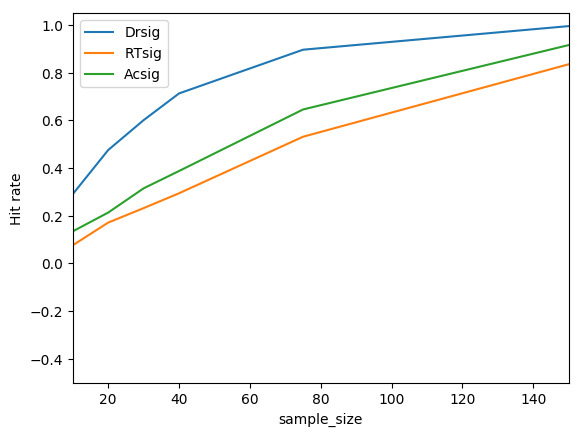
\includegraphics[width=0.68\linewidth]{figs/HitRate} 

}

\caption{Simulated experiment sample size against hit rate (effect size = 2 cohen's d for drift parameter)}\label{fig:vanillahits}
\end{figure}

When the difference in drifts is a Cohen's d of 0, i.e.~no true
difference, we get a false positive rate of \textasciitilde{}0.05 as we
expect, see Figure \ref{fig:vanillaFAs}.

\begin{figure}

{\centering 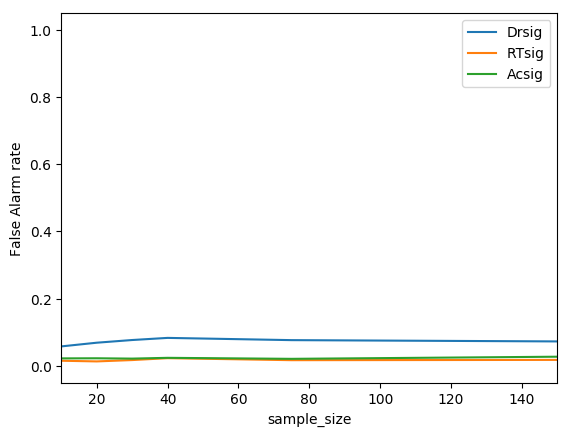
\includegraphics[width=0.68\linewidth]{figs/FalseAlarms} 

}

\caption{Simulated experiment sample size against false positive rate (effect size = 0 cohen'd d for drift parameter)}\label{fig:vanillaFAs}
\end{figure}

To correct for variations in rate of false postives we can calculate d'
(\enquote{d prime}), treating the analysis as if it was a psychophysical
observer. This makes little difference if the false positive rate is
relatively constant, as in this case, but note the d' of drift at the
highest sample size dips due to a rise in the corresponding false
positive rate (probably just a random fluctation due to relatively small
sample sizes). See Figure \ref{fig:vanilladprime}

\begin{figure}

{\centering 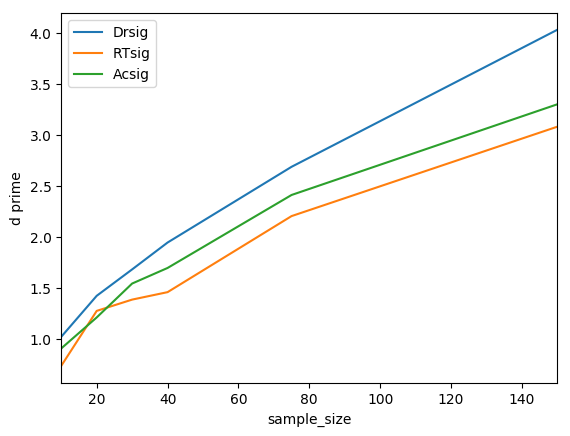
\includegraphics[width=0.68\linewidth]{figs/dprime} 

}

\caption{Simulated experiment sample size against d' (for effect size of 2 vs 0  cohen'd d for drift parameter)}\label{fig:vanilladprime}
\end{figure}

\subsection{With SATOs}\label{with-satos}

The superiority of parameter recovery via a decision model becomes even
more stark if there are systemmatic speed-accuracy trade-offs. To see
this, we re-run the simulatations above, but with a shift in the
boundary parameter before group A and group B, such that individuals
from group B have a lower boundary, and so tend to make faster but less
accurate decisions compared to group B. On top of this difference, we
simulate different sizes of superiority of drift rate of group B over
group A.

For the plots below, the drift rate difference is, as above, 0.1 (which,
given the interindividual variability translates into an effect size of
2). The boundary parameter difference is also 0.1 / effect size 2.

Unlike when there are no SATOs, the reaction time measure is superior
for detecting a group difference than the drift measure, Figure
\ref{fig:SATOhits}.

\begin{figure}

{\centering 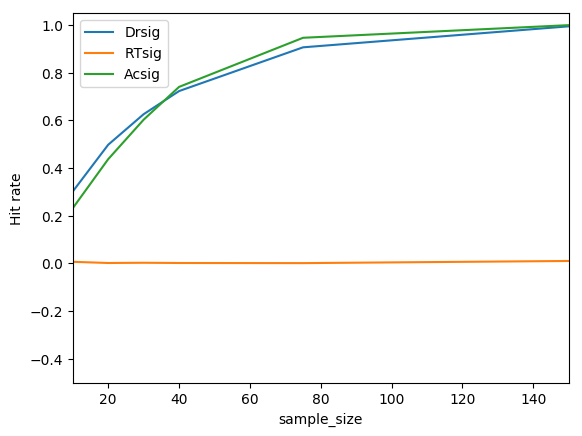
\includegraphics[width=0.68\linewidth]{figs/SATO_HitRate} 

}

\caption{Simulated experiment sample size against hit rate (effect size = 2 cohen's d for drift parameter, 2 for boundary parameter)}\label{fig:SATOhits}
\end{figure}

This, however, is an artifact of the SATO. If the boundary shift had
been in the reverse direction then accuracy, not reaction time, would
appear the superior measure. Once we compare the false positive rate the
danger of using a single observed measure becomes clear, Figure
\ref{fig:SATOFAs}.

\begin{figure}

{\centering 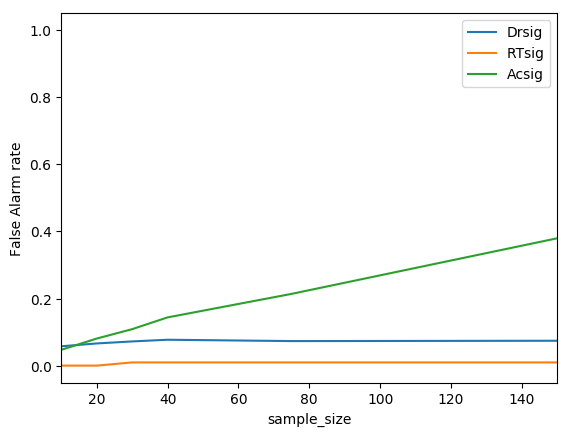
\includegraphics[width=0.68\linewidth]{figs/SATO_FalseAlarms} 

}

\caption{Simulated experiment sample size against false alarm rate (effect size = 2 cohen's d for drift parameter, 2 for boundary parameter)}\label{fig:SATOFAs}
\end{figure}

When using the drift parameter as a measure the SATO between the groups
does not induce false alarms. The accuracy measure is insensitive so
also doesn't suffer (but would if the boundary shift was in the opposite
direction). The reaction time measure is catastrophically sensitive to
false alarms, approaching 100\% false alarm rate with larger samples.

Combining the hit rate and the false alarm rate to calculate d', and so
see measure sensitivity, Figure \ref{fig:SATOdprime}.

\begin{figure}

{\centering 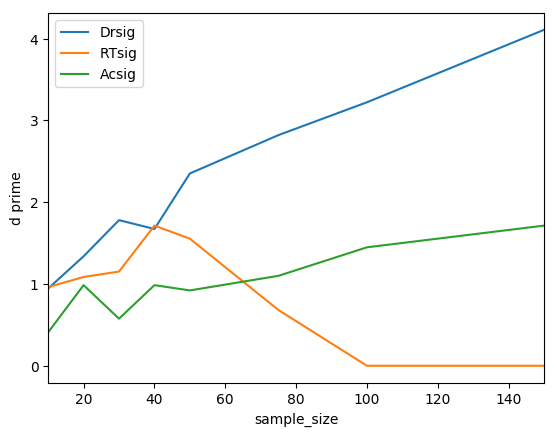
\includegraphics[width=0.68\linewidth]{figs/SATO_dprime} 

}

\caption{Simulated experiment sample size against d' (effect size = 2 cohen's d for drift parameter, 2 for boundary parameter)}\label{fig:SATOdprime}
\end{figure}

\section{Discussion}\label{discussion}

Main conclusions

\begin{itemize}
\item
  Accuracy better than RT (but why?)
\item
  Significant gains for parameter recovery via DDM (e.g.~for 80\% power,
  participants required per group are \textasciitilde{}60 for drift,
  \textasciitilde{}100 for accuracy, \textasciitilde{}150 for RT).
\item
  Signfiicant protection against false positives in the case of between
  groups SATO
\end{itemize}

Results hold only for the (plausible) parameter regime choosen (ie they
are not analytically proved, only numerically demonstrated)

Something about agnosticism between different variations of the the DDM
(ref for this = ?)

\textbf{TODO:}

\begin{itemize}
\tightlist
\item
  Replicate using another decision model (LBA? DMAT?)
\item
  Add literature on SATOs etc
\end{itemize}

\section*{References}\label{references}
\addcontentsline{toc}{section}{References}

\hypertarget{refs}{}
\hypertarget{ref-bruyer2011combining}{}
Bruyer, R., \& Brysbaert, M. (2011). Combining speed and accuracy in
cognitive psychology: Is the inverse efficiency score (ies) a better
dependent variable than the mean reaction time (rt) and the percentage
of errors (pe)? \emph{Psychologica Belgica}, \emph{51}(1), 5--13.

\hypertarget{ref-palmer2005effect}{}
Palmer, J., Huk, A. C., \& Shadlen, M. N. (2005). The effect of stimulus
strength on the speed and accuracy of a perceptual decision.
\emph{Journal of Vision}, \emph{5}(5), 1--1.

\hypertarget{ref-stone2014using}{}
Stone, J. V. (2014). Using reaction times and binary responses to
estimate psychophysical performance: An information theoretic analysis.
\emph{Frontiers in Neuroscience}, \emph{8}, 35.

\hypertarget{ref-wiecki2013hddm}{}
Wiecki, T. V., Sofer, I., \& Frank, M. J. (2013). HDDM: Hierarchical
bayesian estimation of the drift-diffusion model in python.
\emph{Frontiers in Neuroinformatics}, \emph{7}, 14.






\end{document}
